\documentclass[12pt,fleqn]{article}
\setlength{\parindent}{0pt}
\usepackage{graphicx}
\usepackage{cancel}
\usepackage{listings}
\usepackage[latin5]{inputenc}
\usepackage{color}
\setlength{\parskip}{8pt}
\setlength{\parsep}{0pt}
\setlength{\headsep}{0pt}
\setlength{\topskip}{0pt}
\setlength{\topmargin}{0pt}
\setlength{\topsep}{0pt}
\setlength{\partopsep}{0pt}
\setlength{\mathindent}{0cm}
\usepackage{latexsym}
\usepackage{showkeys}
\renewcommand*\showkeyslabelformat[1]{(#1)}

\begin{document}
Ders 1 

Kumeler 

Eger $S$ kumesi ``yukaridan sinirlanmis (bounded from above)'' ise o zaman
$x \in S$ icin oyle bir $y$ var demektir ki her $x$ icin $x \le y$
olsun. Yani $S$ icindeki her deger bu $y$ degerinden kucuk olsun. Bu $x$
degerine $S$'in supremum'u da deniyor, ve $\sup\limits_{x \in S}(x)$ ya da
$sup\{x:x \in S\}$ olarak gosterilebiliyor. Benzer sekilde kumenin en alt
siniri, yani infimum degeri $\inf\limits_{x \in S}(x)$ ya da $inf\{x:x \in
S\}$ olarak gosteriliyor. 

Eger elimizde bir seri (sequence) var ise o zaman sartlari biraz daha
gevsetmek iyidir, burada limit superior kavrami devreye girer. Inf ve sup
degerleri alti / ustu deger olamaz, ama limit superior oyle bir sayidir ki
onun sonrasinda sonlu (finite) / belli sayida kume ogesi olmasina izin
verilir. Limit superior aslinda bir serinin yaklastigi (converge) degerden
baskasi degildir. 

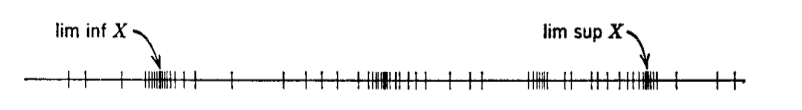
\includegraphics[height=1.5cm]{1_01.png}

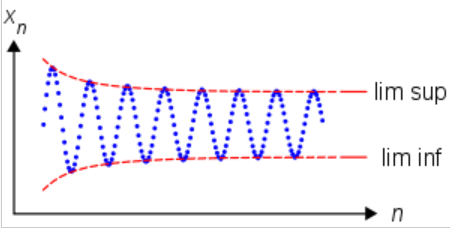
\includegraphics[height=3cm]{1_02.png}

Formel olarak diyelim ki $\{x_n\}$ bir seri, ve diyelim ki bir reel
sayi $S$ var, ki bu reel sayi su sartlari tatmin ediyor 
1) Her $\epsilon > 0$ icin bir $N$ var, oyle ki her $n>N$ icin $x_n
< S + \epsilon$ 
ve 2) her $\epsilon > 0$ ve $M>0$ icin bir  $n>M$ var ki $x_n
> S - \epsilon$. O 
zaman $S$ sayisina  $\{x_n\}$ serisinin limit superior'u denir. 

Bu tanimin soylemeye calistigi serinin yaklastigi degerden sonra ve once
sonlu buyuklukte (bir pencere tanimlarsak bu pencere icinde sonlu sayida
eleman olacaktir (sonsuz degil). Bu pencerenin tanimlanabiliyor olmasi,
onun makul bir noktada olmasini gerektirir, ki bu nokta da yaklasilan
degerden baskasi degildir. 

Limit inferior bunun tersidir, 

\[ \lim \inf x_n  = -\lim \sup(-x_n)\]




















\end{document}
